\documentclass[10pt, a4paper]{article}
\usepackage[english]{babel}
\usepackage[margin=3cm]{geometry}
\usepackage{amsmath}
\usepackage{amsfonts}
\usepackage{amssymb}
\usepackage{listings}
\usepackage{framed}
\usepackage[nottoc]{tocbibind}
\usepackage{booktabs}
\usepackage{url}
\usepackage{graphicx}
\usepackage{subcaption}

\usepackage{booktabs}

\usepackage[utf8]{inputenc}

\usepackage{microtype}

\usepackage{listings}
\usepackage{color}

\lstset{
    belowcaptionskip=1\baselineskip,
    breaklines=true,
    frame=l,
    xleftmargin=\parindent,
    showstringspaces=false,
    basicstyle=\footnotesize\ttfamily,
    keywordstyle=\bfseries,
    commentstyle=\color{cyan}\itshape,
    stringstyle=\ttfamily,
    numbers=left,
    numbersep=5pt,
    numberstyle=\tiny,
}

\setlength{\parindent}{0pt}
\setlength{\parskip}{1em}

\graphicspath{{images/}}

\usepackage{varioref}
\usepackage[plainpages=false,hidelinks]{hyperref}
\usepackage{cleveref}

\begin{document}
\begin{titlepage}

\fontsize{12pt}{14pt}
\selectfont

\begin{center}


\includegraphics[height=3cm]{includes/images/UGent}

\vspace{0.5cm}

Faculty of Engineering\\
Master of Science in Computer Science\\

\vspace{4.0cm}

\fontseries{bx}
\fontsize{17.28pt}{21pt}
\selectfont

\textbf{DESIGN OF MULTIMEDIA APPLICATIONS} \\
\vspace{40pt}

\hrule
\vspace{20pt}
\textsc{Group 40}\\
\vspace{10pt}
\textbf{Report: Error Correction in Digital Video}\\
\vspace{20pt}
\hrule

\vspace{25pt}

\fontseries{m}
\fontsize{12pt}{14pt}
\selectfont

\vspace{5.0cm}

\fontseries{m}
\fontsize{12pt}{14pt}
\selectfont

\hspace{0.5cm} Group 40
\textbf{ 
	\hfill\textsc{Naessens} Tom\\
	\hfill\textsc{Van Den Bossche} Pieter\\
	\hfill\textsc{Wijnant} Joris\\
}
\end{center}
\end{titlepage}

\tableofcontents
\newpage

\thispagestyle{plain}
\section{Gebruikt Vaag Regelsysteem}

Voor de implementatie van het vaag regelsysteem maken we gebruik van de externe bibliotheek jFuzzyLogic~\cite{jfuzzylogic, cingolanijfuzzylogic, cingolani2012jfuzzylogic}. Dit raamwerk stelt ons in staat om op een eenvoudige wijze de lidmaatschapsfuncties op te geven, de t-normen en t-conormen te kiezen, regels te bepalen en samenvoegen en tenslotte de nodige verscherpingen door te voeren. jFuzzyLogic is conform de specificatie van de Fuzzy Control Language (FCL) van IEC werkgroep~\cite{fcl}. 

Alvorens we het raamwerk in gebruik namen, gingen we na of de nodige t-normen en t-conormen, zoals die van \L ukasiewicz, aanwezig zijn. Dit blijkt het geval te zijn, hoewel de benamingen van deze normen verschillen. Zo zal de \L ukasiewicz t-norm als \texttt{BDIF} aangeduid worden met als corresponderende t-conorm is de \texttt{BSUM}. Voor de probabilistische normen vinden we de t-norm \texttt{PROD} en t-conorm \texttt{ASUM}. We kunnen onszelf ervan vergewissen dat deze identiek gedefinieerd zijn als in de cursus en opgave door te kijken naar de specificatie van FCL~\cite{fcl}.

Om discrete lidmaatschapsfuncties te definiëren kunnen we enkele singletons opgeven. Voor continue lidmaatschapsfuncties biedt het raamwerk ons meerdere mogelijkheden. Zo kunnen we een functie definiëren aan de hand van haar knikpunten, of aan de hand van ingebouwde functies voor enkele voorgedefinieerde vormen zoals triangulaire of trapezoïdale lidmaatschapsfuncties. De linguïstische termen die over hetzelfde universum en dezelfde invoer gedefinieerd zijn zullen ook samengevoegd zijn in blokken.

Het opstellen van regels is ook zeer eenvoudig aan de hand van \emph{rule blocks}. Deze blokken omvatten een aantal regels onder de vorm van linguïstische uitdrukkingen. Hierbij kunnen de binaire operatoren \texttt{AND}, \texttt{OR} en de unaire operator \texttt{NOT} gebruikt worden die respectievelijk de t-norm, t-conorm en het complement zullen toepassen. De normen die gebruikt moeten worden voor de regels in het blok worden aan het begin van het blok opgegeven. Ook de normen die gebuikt worden voor de bepaling van de samenvoeging van regels wordt hier vastgelegd voor het blok.

Voor de verscherping gebruiken we de formule die in de opgave vermeldt staat. Deze is in het raamwerk bekend als de Centre of Gravity (COG) formule. Deze zal het zwaartepunt van de samengevoegde vaagverzamelingen nemen, zoals dus gevraagd wordt in de opgave. De alternatieven die het raamwerk verder ook aanbiedt zijn Right Most Maximum (RM) en Left Most Maximum (LM). Deze laatste zullen resulteren in respectievelijk een hogere en lagere waarde ten opzichte van de COG formule. De gebruikte methode moeten we in het raamwerk per uitvoer opgegeven.

\section{Implementatie Controllers}
In deze sectie overlopen we de assumpties die we hebben gemaakt over het gedrag van 
de wagen en welke bewerkingen we toegepast hebben op de invoerdata van het vage 
raamwerk. Daarna bekijken we kort de algemene lidmaatschapsfuncties, waarna we 
dieper ingaan op de specifieke implementatie van de drie verschillende 
controllers. Tenslotte kijken we naar de eventuele verschillen in de lidmaatschapsfuncties voor de individuele controllers.

\subsection{Regels}

Om de wagen doorheen de parcours te leiden hebben we enkele beschouwingen gemaakt over het gedrag van de wagen.

Ten eerste zien we dat er twee mogelijke denkwijzen zijn voor het sturen van de wagen. Ofwel laten we de wagen wegsturen van de randen van het parcours, ofwel laten we de wagen in de richting rijden naar waar deze het verste kan kijken. De eerste zal steeds een veilige route kiezen die een minimumafstand behoudt tot de grenzen van het parcours. De tweede zal echter meer sportief de binnenkant van de bocht nemen. Dit maakt de eerste manier van sturen meer geschikt voor de veilige controller terwijl de tweede voor de snelle en drift controller interessanter is.

We merken ook op dat wanneer de snelheid van de wagen omhoog gaat, de remafstand ook hoger ligt. We moeten dus ervoor zorgen dat de wagen bij hogere snelheden ook sneller zal beginnen remmen. Daarnaast kunnen bruuske bewegingen bij hoge snelheden ervoor zorgen dat de wagen begint te slippen. We zullen dus aan de hand van de sensor vooraan de wagen in combinatie met de snelheid nagaan wanneer de wagen moet beginnen remmen.

Wanneer de wagen een bocht nadert zal deze moeten vertragen. Wanneer we de 
tweede manier van sturen gebruiken, kijken we naar waar de wagen moet gaan. 
Hierbij kan een problematisch randgeval zich voordoen indien de sensoren aan 
beide zijden van de wagen ongeveer dezelfde waarden aangeven. In dit geval zullen de regels voor het sturen niet kunnen vaststellen in welke richting er gestuurd moet worden. Daarom zullen we 
de hoek van deze sensoren aanpassen indien de afstanden tot zowel de voor- als 
zij-sensoren te klein worden.

Indien de wagen begint te slippen willen we dat deze zich zal stabiliseren. We zullen in dit geval dus de versnelling van de wagen stoppen en stilaan remmen. Indien we te bruusk remmen of versnellen tijdens het remmen zullen we harder aan het slippen gaan, wat zeker niet de bedoeling is voor de veilige en snelle controllers.

Tenslotte moeten we rekening houden met de baanbreedte in combinatie met de afstanden die beide
zij-sensoren ons geven. Op het circuit van Texas zijn er bijvoorbeeld heel lange, maar ook heel
brede bochten. In Silverstone en Spa-Francorchamps is de baan daarentegen heel smal en zijn de
bochten zeer scherp. We kunnen dus niet puur afgaan op de afstanden die de
zij-sensoren aangeven om bochten op alle parcoursbreedtes te herkennen. We zullen dit moeten oplossen door deze
afstand te normaliseren. Daarom voeren we eerst een bewerking door op deze sensoren
die als resultaat een genormaliseerde waarde tussen $-1$ en $1$ oplevert, dit
resultaat noemen we \texttt{corner}. $-1$ komt overeen met een scherpe bocht
naar links, $1$ met een scherpe bocht naar rechts. Wanneer de wagen op een recht
stuk zit en dus beide zij-sensoren een gelijke waarde aangeven is het resultaat
$0$. Negatieve waarden tussen $-1$ en $0$ geven bochten naar links aan, waarbij
lagere waarden scherpere bochten zijn. Het inverse geld ook voor bochten naar
rechts. Op basis van deze \texttt{corner} waarde kunnen we dan verschillende
linguïstische termen vastleggen om scherpe, gewone en milde bochten aan te geven.

\subsection{Lidmaatschapsfuncties}

Voor de verschillende controllers gebruiken we andere lidmaatschapsfuncties. Dit 
doen we omdat bijvoorbeeld voor de veilige controller een trage snelheid lager 
zal liggen dan die in de snelle controller. Om makkelijk de vergelijking te maken hebben we de invoeren uitgezet in Figuur~\ref{fig:lidfties_in} en de uitvoeren in Figuur~\ref{fig:lidfties_out}.

\begin{figure}[h]
\centering
% KPH
  \begin{subfigure}[b]{0.32\textwidth}
    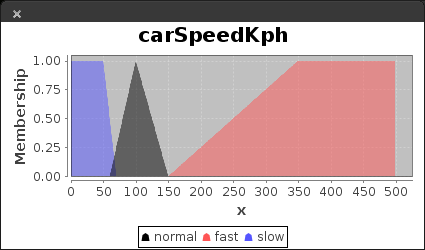
\includegraphics[width=\textwidth]{safe/carSpeedKph}
  \end{subfigure}%
  ~
  \begin{subfigure}[b]{0.32\textwidth}
    \includegraphics[width=\textwidth]{speed/carSpeedKph}
  \end{subfigure}%
   ~
  \begin{subfigure}[b]{0.32\textwidth}
    \includegraphics[width=\textwidth]{rally/carSpeedKph}
  \end{subfigure}\\
% Corner
  \begin{subfigure}[b]{0.32\textwidth}
    \includegraphics[width=\textwidth]{safe/corner}
  \end{subfigure}%
  ~
  \begin{subfigure}[b]{0.32\textwidth}
    \includegraphics[width=\textwidth]{speed/corner}
  \end{subfigure}%
   ~
  \begin{subfigure}[b]{0.32\textwidth}
    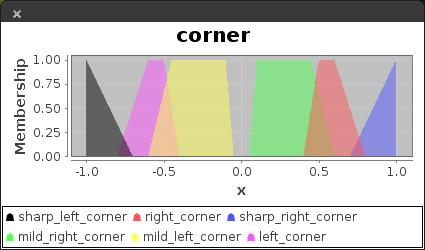
\includegraphics[width=\textwidth]{rally/corner}
  \end{subfigure}\\
% lateralVelocity
  \begin{subfigure}[b]{0.32\textwidth}
    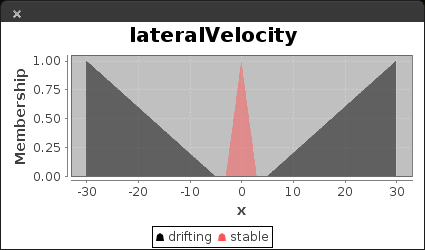
\includegraphics[width=\textwidth]{safe/lateralVelocity}
  \end{subfigure}%
  ~
  \begin{subfigure}[b]{0.32\textwidth}
    \includegraphics[width=\textwidth]{speed/lateralVelocity}
  \end{subfigure}%
   ~
  \begin{subfigure}[b]{0.32\textwidth}
    \includegraphics[width=\textwidth]{rally/lateralVelocity}
  \end{subfigure}\\  
% frontSensor
  \begin{subfigure}[b]{0.32\textwidth}
    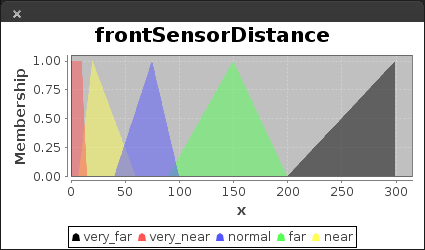
\includegraphics[width=\textwidth]{safe/frontSensor}
    \caption{Veilig}
    \label{fig:safe_in}
  \end{subfigure}%
  ~
  \begin{subfigure}[b]{0.32\textwidth}
    \includegraphics[width=\textwidth]{speed/frontSensor}
    \caption{Snel}
    \label{fig:speed_in}
  \end{subfigure}%
   ~
  \begin{subfigure}[b]{0.32\textwidth}
    \includegraphics[width=\textwidth]{rally/frontSensor}
    \caption{Drift}
    \label{fig:drift_in}
  \end{subfigure}\\ 
\caption{Lidmaatschapfuncties invoer}\label{fig:lidfties_in}
\end{figure}

\begin{figure}[h]
\centering
% Accel
  \begin{subfigure}[b]{0.32\textwidth}
    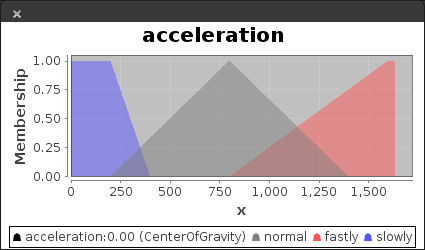
\includegraphics[width=\textwidth]{safe/acceleration}
  \end{subfigure}%
  ~
  \begin{subfigure}[b]{0.32\textwidth}
    \includegraphics[width=\textwidth]{speed/acceleration}
  \end{subfigure}%
   ~
  \begin{subfigure}[b]{0.32\textwidth}
    \includegraphics[width=\textwidth]{rally/acceleration}
  \end{subfigure}\\
% Brake
  \begin{subfigure}[b]{0.32\textwidth}
    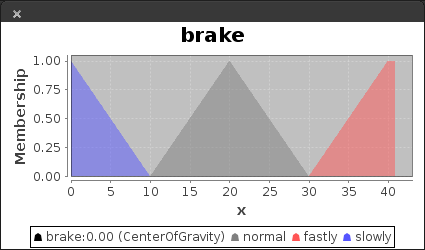
\includegraphics[width=\textwidth]{safe/brake}
  \end{subfigure}%
  ~
  \begin{subfigure}[b]{0.32\textwidth}
    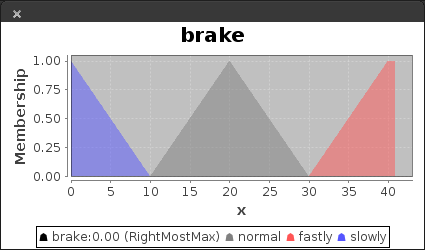
\includegraphics[width=\textwidth]{speed/brake}
  \end{subfigure}%
   ~
  \begin{subfigure}[b]{0.32\textwidth}
    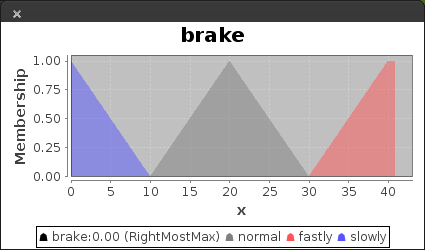
\includegraphics[width=\textwidth]{rally/brake}
  \end{subfigure}\\
% steering
  \begin{subfigure}[b]{0.32\textwidth}
    \includegraphics[width=\textwidth]{safe/steering}
  \end{subfigure}%
  ~
  \begin{subfigure}[b]{0.32\textwidth}
    \includegraphics[width=\textwidth]{speed/steering}
  \end{subfigure}%
   ~
  \begin{subfigure}[b]{0.32\textwidth}
    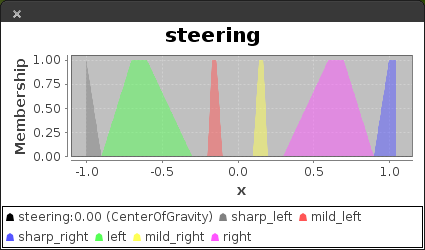
\includegraphics[width=\textwidth]{rally/steering}
  \end{subfigure}\\
% scanAngle
  \begin{subfigure}[b]{0.32\textwidth}
    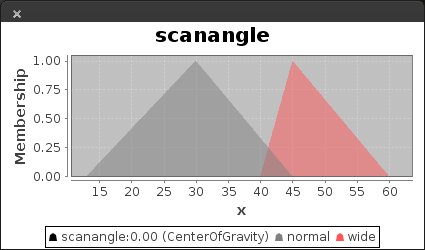
\includegraphics[width=\textwidth]{safe/scanAngle}
    \caption{Veilig}
    \label{fig:safe_out}
  \end{subfigure}%
  ~
  \begin{subfigure}[b]{0.32\textwidth}
    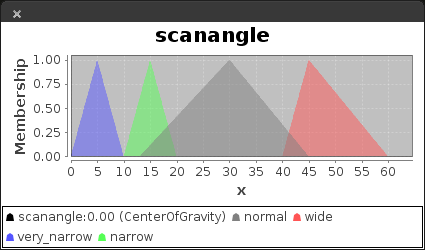
\includegraphics[width=\textwidth]{speed/scanAngle}
    \caption{Snel}
    \label{fig:speed_out}
  \end{subfigure}%
   ~
  \begin{subfigure}[b]{0.32\textwidth}
    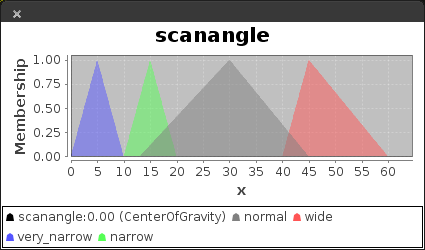
\includegraphics[width=\textwidth]{rally/scanAngle}
    \caption{Drift}
    \label{fig:drift_out}
  \end{subfigure}\\
\caption{Lidmaatschapfuncties uitvoer}\label{fig:lidfties_out}
\end{figure}

We gebruiken de volgende invoeren:
\begin{itemize}
\item \texttt{\textbf{carSpeedKph:}} De snelheid van de wagen in km/h.
\item \texttt{\textbf{frontSensorDistance:}} De afstand van de voorkant van wagen tot de muur in meter.
\item \texttt{\textbf{corner:}} Intensiteit van de bocht, gaande van $-1$ voor een scherpe bocht naar links tot $1$ voor een scherpe bocht naar rechts. 
\item \texttt{\textbf{lateralVelocity:}} De zijwaartse snelheid van de wagen die aangeeft of de wagen al dan niet slipt.
\end{itemize}

En leggen de volgende uitvoeren vast in functie van deze invoeren:
\begin{itemize}
\item \texttt{\textbf{acceleration:}} De versnelling van de wagen van $0$ tot $1600$. Indien er geen waarde berekend wordt zal deze $0$ zijn. Deze is voor alle controllers opgedeeld in enkele termen die overeenkomen met een lage ( \texttt{slowly}), gematigde (\texttt{normal}) en snelle (\texttt{fastly}) acceleratie.
\item \texttt{\textbf{brake:}} Geeft aan hoe hard de wagen dient te remmen. Indien er geen waarde berekend wordt zal deze $0$ zijn. Deze is eveneens voor alle controllers opgedeeld in 3 termen: \texttt{slowly}, \texttt{normal} en \texttt{fastly}.
\item \texttt{\textbf{steering:}} De richting en hoe scherp er gestuurd moet worden. Deze waarde zal van $-1$ tot $1$ gaan, analoog aan de corner invoer.
\item \texttt{\textbf{scanangle:}} geeft aan wat de nieuwe hoek van de 
zijsensoren wordt. Bij de safecontroller werken we enkel met \texttt{normal} en 
\texttt{wide}, maar bij de speed- en driftcontroller breiden we deze uit met 
\texttt{narrow} en \texttt{very\_narrow} om verder vooruit te kunnen kijken.
\end{itemize}

De overige gegevens worden niet gebruikt, of worden enkel gebruikt voor de 
berekening van de inputs zoals de zij-sensoren die worden gecombineerd en 
genormaliseerd tot \texttt{corner}.

Merk op voor de uitvoer \emph{brake} dat de termen disjunct zijn in onze controllers waardoor de COG methode het gemiddelde van deze gebieden zou geven. Om ervoor te zorgen dat deze waarden toch worden opgetrokken zullen we dus in plaats van de COG formule de RM formule gebruiken in de snellere controllers. Volgens een analoge redenering hebben we geopteerd om de RM functie te gebruiken voor de acceleratie.

Alternatief hadden we deze termen discreet kunnen maken aan de hand van singletons. Hierdoor zouden we een exacte waarde kunnen opleggen aan de uitvoer. Hierdoor zou de impact van een vaag regelsysteem te gebruiken echter afgezwakt worden en zouden de controllers dus gevoeliger worden voor kleine veranderingen in de invoer.

\subsection{Veiligheid}
De veilige implementatie is een zeer eenvoudige implementatie. Om uiterst veilig
te zijn rijden we niet veel sneller dan 70 km/h, wat overeen komt met de boven grens van de term \texttt{slow} voor deze controller. Bochten nemen we afhankelijk van hun scherpte. Scherpe bochten nemen we scherp, gewone bochten nemen we
normaal en milde bochten sturen we mild in. We versnellen enkel snel wanneer de
auto traag rijdt, en remmen doen we snel wanneer een bocht binnenrijden en doen
we gestaag wanneer een bocht in de verte aankomt. Wanneer we een bocht naderen
zetten we als laatste de zij-sensoren iets wijder om een beter zicht op het soort
bocht te krijgen.

De lidmaatschapsfuncties van deze controllers is te vinden in de de linkerkolommen 
van figuren \ref{fig:lidfties_in} en \ref{fig:lidfties_out}.

Dit resulteert in de volgende regelblokken:

\begin{lstlisting}
RULEBLOCK steering
  RULE 1 : IF corner IS sharp_left_corner THEN steering IS sharp_left;
  RULE 2 : IF corner IS left_corner THEN steering IS left;
  RULE 3 : IF corner IS mild_left_corner THEN steering IS mild_left;
  RULE 4 : IF corner IS mild_right_corner THEN steering IS mild_right;
  RULE 5 : IF corner IS right_corner THEN steering IS right;
  RULE 6 : IF corner IS sharp_right_corner THEN steering IS sharp_right;
END_RULEBLOCK

RULEBLOCK speedup
  RULE 1 : IF carSpeedKph IS slow THEN acceleration IS fastly;
END_RULEBLOCK

RULEBLOCK brake
  RULE 1 : IF frontSensorDistance IS normal THEN brake IS normal;
  RULE 2 : IF frontSensorDistance IS near THEN brake IS fastly;
END_RULEBLOCK

RULEBLOCK scanangle
  RULE 1: IF frontSensorDistance is near THEN scanangle IS wide;
END_RULEBLOCK
\end{lstlisting}
\subsection{Snelheid}
We nemen voornamelijk de lidmaatschapsfuncties over van de veilige controller, maar moeten hier wel wat 
aanpassingen maken. De veilige controller versnelde nooit boven de 70 km/h. 
Daardoor moesten we geen rekening houden met hoge snelheden en dus grotere remafstanden. Met de snelle controller mikken we op hogere snelheden en zullen we dus wel moeten doen. Daarom voegen we enkele termen toe bij de 
\texttt{carSpeedKph}-invoer om op grotere snelheden te kunnen anticiperen. Deze termen zijn \texttt{very\_fast} en \texttt{hyper\_fast}. Merk hierbij op dat deze nieuwe vaagverzamelingen inclusief zijn ten opzichte van de vaagverzameling die overeen komt met de term \texttt{fast}. Dit doen we omdat we willen dat wanneer we zeer snel gaan dit nog steeds als snel beschouwd kan worden. Bovendien is de term \texttt{hyper\_fast} sterk inclusief omdat deze in de kern van de term \texttt{fast} omvat is. Voor \texttt{very\_fast} hebben we geen sterke inclusie tegenover \texttt{fast} omdat deze eerste een klein gebied buiten de kern van de laatste omvat.

Door de hogere snelheden is het belangrijk om ervoor te zorgen dat de wagen stabiel blijft. Daarom zullen we een nieuwe term toevoegen voor de \texttt{lateralVelocity}-invoer. Deze nieuwe term, \texttt{minimal}, zal aangeven dat de wagen niet alleen stabiel is maar zeer stabiel. In dit geval zal het mogelijk zijn om sterk te versnellen zonder te beginnen slippen. Daarnaast kunnen we door de verhoogde snelheid ook hogere laterale snelheden verwachten. Om deze op te vangen moeten we de lidmaatschapsfunctie van de term \texttt{drifting} uitbreiden.

Om de langere remafstanden die met deze hogere snelheden gepaard gaan moeten we vervolgens ook aanpassingen doorvoeren op de lidmaatschapsfuncties van de termen voor de \texttt{frontSensorDistance}-invoer. Hierbij zullen we geen gebruik meer maken van de term \texttt{very\_near}, waardoor we deze kunnen weglaten. Belangrijker voor deze controller is het correct inschatten van de remafstand. Derhalve breiden we de termen \texttt{far} en \texttt{very\_far} uit tot maximaal 1000 meter. Ook hier zullen we analoog aan de snelheid de term \texttt{very\_far} sterk inclusief maken ten opzichte van de term \texttt{far}.

Voor de uitvoer zullen we slechts beperkte aanpassingen moeten doen. Zo zullen we de acceleratie en het remgedrag iets scherper stellen door in plaats van de COG functie de RM functie te gebruiken. Ook verschuiven we het zwaartepunt door de grenzen tussen de termen strenger te maken.

Als laatste aanpassing aan de lidmaatschapsfuncties laten we de wagen sneller bochten ontdekken door de de \texttt{scanangle} uitvoer toe te staan te vernauwen. Dit zal gebeuren wanneer de wagen voldoen de ver kan kijken of zeer hoge snelheden haalt. Dit zal ervoor zorgen dat de wagen in mindere mate heen en weer zal schommelen bij hoge snelheden. De regels die hieruit voortvloeien staan in het \texttt{scanangle} rule-block.

De bekomen lidmaatschapsfuncties van deze controller voor de uitvoer zijn te vinden in de 
middelste kolom van Figuur~\ref{fig:lidfties_in}. De invoer is terug te vinden in dezelfde kolom van Figuur~\ref{fig:lidfties_out}.

Bij het opstellen van de regels moeten we een afweging maken tussen snelheid en 
veiligheid. We moeten snel rijden op lange stukken, maar ook rekening houden 
met de langere remweg die dit met zich meebrengt. Aan grote snelheid hebben 
kleine stuurcorrecties ook veel meer impact, dus we moeten ervoor zorgen dat we 
bij het uitvoeren van die correcties onze snelheid verlagen en niet 
versnellen tijdens deze manoeuvres om de controle over het stuur niet te 
verliezen.

Aan de regels voor de besturing van de veilige controller, in het \texttt{steering} rule-block, hebben we geen aanpassingen gedaan omdat we ervoor zorgen dat de wagen voldoende vertraagt wanneer deze een bocht nadert met de regels in het \texttt{brake} rule-block.

\begin{lstlisting}
RULEBLOCK steering
  RULE 1 : IF corner IS sharp_left_corner THEN steering IS sharp_left;
  RULE 2 : IF corner IS left_corner THEN steering IS left;
  RULE 3 : IF corner IS mild_left_corner THEN steering IS mild_left;
  RULE 4 : IF corner IS mild_right_corner THEN steering IS mild_right;
  RULE 5 : IF corner IS right_corner THEN steering IS right;
  RULE 6 : IF corner IS sharp_right_corner THEN steering IS sharp_right;
END_RULEBLOCK

RULEBLOCK speedup
  RULE 1 : IF carSpeedKph IS slow AND lateralVelocity IS stable  AND 
  frontSensorDistance IS near THEN acceleration IS slowly;
  RULE 2 : IF (carSpeedKph IS slow OR carSpeedKph IS normal) AND 
  lateralVelocity IS stable  AND 
  frontSensorDistance IS far THEN acceleration IS fastly;

  RULE 4 : IF carSpeedKph IS fast AND lateralVelocity IS minimal AND 
  frontSensorDistance IS very_far THEN acceleration IS fastly;
  RULE 5 : IF carSpeedKph IS hyper_fast AND frontSensorDistance IS NOT very_far 
  THEN acceleration IS slowly;
END_RULEBLOCK

RULEBLOCK brake
  RULE 1 : IF lateralVelocity IS drifting AND carSpeedKph IS slow THEN brake IS 
  slowly;
  RULE 2 : IF lateralVelocity IS drifting AND carSpeedKph IS NOT slow THEN 
  brake IS fastly;

  RULE 3 : IF frontSensorDistance IS near AND carSpeedKph IS normal THEN brake 
  IS normal;

  RULE 4 : IF frontSensorDistance IS NOT far AND carSpeedKph IS fast THEN brake 
  IS slowly;
  RULE 5 : IF frontSensorDistance IS NOT very_far AND carSpeedKph IS very_fast 
  THEN brake IS fastly;
  RULE 6 : IF carSpeedKph IS fast AND lateralVelocity IS NOT minimal THEN brake 
  IS normal;
  RULE 7 : IF carSpeedKph IS very_fast AND frontSensorDistance IS NOT very_far 
  THEN brake IS fastly;
END_RULEBLOCK

RULEBLOCK scanangle
  RULE 1: IF frontSensorDistance is near THEN scanangle IS wide;
  RULE 2: IF carSpeedKph IS very_fast THEN scanangle IS narrow;
  RULE 3: IF carSpeedKph IS hyper_fast THEN scanangle IS very_narrow;
END_RULEBLOCK

\end{lstlisting}
\subsection{Drift}
De driftcontroller is een meer gewaagde versie van de speedcontroller, waarbij 
er drie algemene aanpassingen zijn gebeurd. Onderstaande beschrijven we onze 
aanpassingen tegenover de hierboven besproken speedcontroller.

Ten eerste hebben we het sturen bruusker gemaakt. Hiervoor hebben we zowel de
lidmaatschapsfuncties van de termen voor \texttt{steering} iets meer richting de extremen gezet.
We hebben ook de steering regels aangepast zoals in onderstaande regelblokken te zien
zijn. In plaats van gewoon naar links te sturen in een gewone linkse bocht
oversturen we eigenlijk. Idem voor rechts. Deze toevoegingen zorgen ervoor dat
we eigenlijk té veel insturen in een bocht, waardoor de achterkant van de auto
zal uitbreken en we beginnen driften.

Dit driften moeten we natuurlijk ook tegengaan om de auto na het oversturen in
een bocht te stabiliseren. Hiervoor voegen we twee nieuwe regels toe, regel 7 en
8 in het \texttt{steering} ruleblock. Wanneer we in een bocht aan het driften
zijn zal de \texttt{corner} variabele uit deze bocht willen sturen, wat
automatisch al betekent dat de auto zal tegensturen. Dus, als we aan het driften
zijn, en de zij-sensoren zien een niet te scherpe bocht naar links/rechts dan
kunnen we concluderen dat we net hebben overstuurd in een bocht naar
rechts/links. Om dit te corrigeren sturen we in dit geval dus scherp in de bocht
die gezien wordt om het oversturen in de originele bocht tegen te gaan.

Een tweede algemene aanpassing die we hebben gemaakt is het weghalen van 
braking-rules. Om een deftige drift te kunnen uitvoeren moeten we met voldoende 
snelheid in de bocht gaan, anders breekt de achterkant van de auto niet uit. We 
willen ook niet extra gaan remmen tijdens het driften, dus ook deze regels 
halen we weg. 

Als laatste willen we uit op het eind van een drift ook extra gas geven om snel 
weg te rijden (en om wat extra rook te ontwikkelen), dus ook hiervoor is een 
extra regel toegevoegd.

De lidmaatschapsfuncties van deze controllers is te vinden in de rechterkolom 
van figuren \ref{fig:lidfties_in} en \ref{fig:lidfties_out}.

\begin{lstlisting}
RULEBLOCK steering
  RULE 1 : IF corner IS sharp_left_corner THEN steering IS sharp_left;
  RULE 2 : IF corner IS left_corner THEN steering IS sharp_left;
  RULE 3 : IF corner IS mild_left_corner THEN steering IS mild_left;
  RULE 4 : IF corner IS mild_right_corner THEN steering IS mild_right;
  RULE 5 : IF corner IS right_corner THEN steering IS sharp_right;
  RULE 6 : IF corner IS sharp_right_corner THEN steering IS sharp_right;

  RULE 7 : IF lateralVelocity IS drifting AND (corner IS mild_right_corner OR 
  corner IS right_corner) THEN steering IS sharp_right;
  RULE 8 : IF lateralVelocity IS drifting AND (corner IS mild_left_corner  OR 
  corner IS left_corner)  THEN steering IS sharp_left;
END_RULEBLOCK

RULEBLOCK speedup
  RULE 1 : IF carSpeedKph IS slow AND frontSensorDistance IS near THEN 
  acceleration IS fastly;
  RULE 2 : IF carSpeedKph IS slow AND frontSensorDistance IS far THEN 
  acceleration IS fastly;
  RULE 3 : IF carSpeedKph IS normal AND frontSensorDistance IS far THEN 
  acceleration IS fastly;

  RULE 4 : IF carSpeedKph IS fast AND lateralVelocity IS minimal AND 
  frontSensorDistance IS very_far THEN acceleration IS fastly;
  RULE 5 : IF carSpeedKph IS hyper_fast AND frontSensorDistance IS NOT very_far 
  THEN acceleration IS slowly;

  RULE 6 : IF lateralVelocity IS drifting THEN acceleration IS fastly;
END_RULEBLOCK

RULEBLOCK brake
  RULE 4 : IF frontSensorDistance IS NOT far AND carSpeedKph IS fast THEN brake 
  IS slowly;
  RULE 5 : IF frontSensorDistance IS NOT very_far AND carSpeedKph IS very_fast 
  THEN brake IS normal;
  RULE 6 : IF carSpeedKph IS fast THEN brake IS normal;
  RULE 7 : IF carSpeedKph IS very_fast AND frontSensorDistance IS NOT very_far 
  THEN brake IS fastly;
END_RULEBLOCK

RULEBLOCK scanangle
  RULE 1: IF frontSensorDistance is near THEN scanangle IS wide;
  RULE 2: IF carSpeedKph IS very_fast THEN scanangle IS narrow;
  RULE 3: IF carSpeedKph IS hyper_fast THEN scanangle IS very_narrow;
END_RULEBLOCK
\end{lstlisting}

\section{Performantie van de Controllers}
\label{sec:performance}
Laten we nu de performantie van onze controllers beschouwen. We kijken hierbij naar de gemiddelde snelheid, topsnelheid, neiging tot driften en hoe robuust de controller is. We geven hierbij ook aan welke circuits de controllers al dan niet kunnen afleggen. In Tabel~\ref{tbl:controllerresultaten} lijsten we de beste resultaten op van de algemene controllers. Bij het produceren van deze resultaten liepen de wagens geen schade op.

\begin{table}
	\centering
	\caption{Beste resultaten van algemene controllers}
	\label{tbl:controllerresultaten}
	
	\begin{subtable}{\linewidth}
   		\centering
   		\caption{Safecontroller}
   		\label{tbl:resultssafe}
       	\begin{tabular}{lrrrr}
        	\toprule
        	Track             & Tijd (s) & Drift (m) & Drift (s) & Top speed 
        	(km/h) \\
        	\midrule
        	Interlagos        & 233.141 & 0 & 0 & 72.06 \\ 
        	Texas             & 121.763 & 0 & 0 & 71.24 \\
        	Spa-Francorchamps &       / & / & / & / \\
        	Silverstone       & 178.367 & 0 & 0 & 71.91 \\
        	\bottomrule
    	\end{tabular}
   	\end{subtable}
   	
	\begin{subtable}{\linewidth}
   		\centering
   		\caption{Speedcontroller}
   		\label{tbl:resultsspeed}
   		\begin{tabular}{lrrrr}
    		\toprule
        	Track             & Tijd (s) & Drift (m) & Drift (s) & Top speed  
        	(km/h) \\
        	\midrule
        	Interlagos        & 128.100 &      0 &     0 & 304.16 \\
        	Texas             &  59.369 & 257.11 & 4.799 & 352.73 \\
        	Spa-Francorchamps &       / &      / &     / &      / \\
        	Silverstone       & 106.700 &   20.5 & 1.600 & 270.97 \\
        	\bottomrule
    	\end{tabular}
   	\end{subtable}
  	   	
   	\begin{subtable}{\linewidth}
   		\centering
   		\caption{Driftcontroller}
   		\label{tbl:resultsdrift}
   	    \begin{tabular}{lrrrr}
   	    \toprule
       	Track             & Tijd (s) & Drift (m) & Drift (s) & Top speed  
       	(km/h) \\
   	    \midrule
       	Interlagos        & 116.081 & 117.29 & 4.342 & 244.47 \\
       	Texas             &  58.034 & 277.37 & 5.000 & 336.69 \\
       	Spa-Francorchamps &       / &      / &     / &      / \\
       	Silverstone       & 109.533 &  66.42 & 2.767 & 272.75 \\
   	    \bottomrule
   	    \end{tabular}
   	\end{subtable}
\end{table}

In de tabel zien we dat er geen gegevens beschikbaar zijn voor het circuit van Spa-Francorchamps. Geen enkele controller was namelijk in staat om door de laatste bocht te raken. Deze bocht is namelijk scherper dan 150 graden (zie Figuur~\ref{fig:spa}) waardoor de zijwaartse scanners niet kunnen uitmaken in welke richting de bocht gaat. Doordat onze controller steeds in de richting rijdt waarheen deze het verste kan kijken zal deze dus beslissen om rechtdoor te gaan, tegen de muur. Hierna zal deze de bocht ook niet meer verlaten.

\begin{figure}[h]
\centering
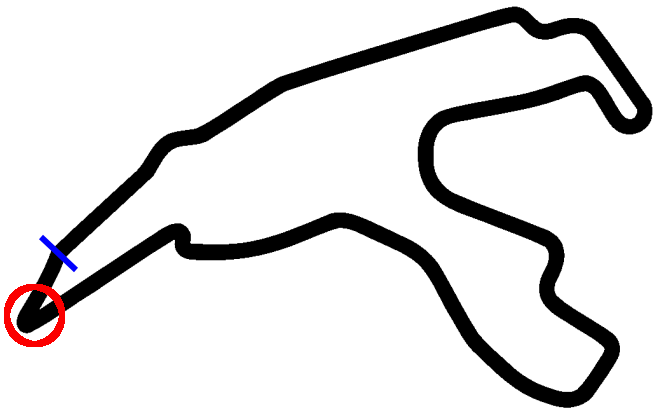
\includegraphics[width=.5\textwidth]{spa_circuit_bocht}
\caption{Circuit van Spa-Francorchamps met de laaste bocht aangeduid met rood}\label{fig:spa}
\end{figure}

De controllers presteren in het algemeen het beste op banen die breed zijn en 
egale bochten hebben, zoals Texas en Interlagos. Op een circuit zoals 
Silverstone en Spa-Francorchamps waar enkele zeer scherpe bochten en scherpe 
slaloms in verwerkt zijn moeten we voorzichtiger rijden met de speedcontroller en durft de driftcontroller al eens uit de bocht te gaan.

\subsection{Veiligheid}

In het geval van de veilige controller zien we dat deze de gemiddelde snelheid 
begrenst wordt tot de bovengrens van \texttt{slow}. Op de rechte stukken 
spreken we hier dus van een topsnelheid van ongeveer 70 km/h. Wanneer deze 
controller bochten tegenkomt zal deze remmen. De snelheid daalt hierbij dan 
daar 50 km/h. Dit trage gedrag zien we duidelijk in Tabel~\ref{tbl:resultssafe} 
aan de rondetijden. Ook zal er bij deze lagere snelheden geen mogelijkheid zijn 
om te driften. 

Verder zal door onze manier van sturen ertoe leiden dat de wagen zelfs op rechte stukken kleine correcties probeert te maken. Dit zou opgevangen moeten worden door het vage regelsysteem maar dit is niet voldoende het geval. Volgens ons is dit te wijten aan \texttt{corner}-invoer. Deze zal namelijk zeer snel aangeven dat er een milde bocht is. Daarnaast zijn de randen van het parcours grillig, wat er nog sneller voor zal zorgen dat de controller beslist om bij te sturen.

Doordat we onze sturing baseren op een locatie die een eind voor de wagen ligt zullen we ook niet naar het midden van de baan sturen maar naar het midden van de baan in de verte. Concreet zal de wagen dus meer naar de binnenkant van de bocht neigen.

De veilige controller blijkt zeer robuust te zijn. De lijn die deze controller doorheen het parcours zal nemen is bijna exact dezelfde doordat de snelheid van de wagen ook steeds dezelfde zal zijn.
\subsection{Snelheid}
De snelle controller is in staat om de circuits van Silverstone en Interlagos af
te leggen zonder te crashen. De snelheid zal hier vari\"eren van 80
km/h in de bochten tot 130 km/h op de rechte stukken. Bij lange rechte stukken
is het mogelijk dat de wagen hogere snelheden behaalt, de topsnelheid die wij op
deze circuits waargenomen hebben is $304.16$ km/h.

Op het snelle circuit van Texas zal de controller zeer hoge snelheden behalen
maar niet op tijd beginnen remmen. De controller zal dus tegen een hoge snelheid
de bocht proberen nemen en bijgevolg slippen en crashen of een lus maken. Ondanks de crash zal
deze controller zeer snelle tijd neerzetten op het circuit. De topsnelheid die we hier meten is $352.73$ km/h.

Zoals we in Tabel~\ref{tbl:resultsspeed} kunnen zien zal de snelle controller ook aanleg hebben tot driften maar zal hier niet op doelen. Zo zien we dat deze op het circuit van Interlagos zijn snelste ronde neerzet zonder te driften. Ook op Silverstone blijft de drift beperkt. Door de crash in Texas zal hier natuurlijk een hoge driftscore verschijnen.

De robuustheid van deze controller ligt al een stuk lager dan die van de veilige controller. Wanneer de wagen namelijk uit een bocht komt en een lang recht stuk nadert, zal de wagen enkel sterk versnellen indien de wagen op tijd stabiel genoeg is. Indien de wagen maar net stabiel genoeg is zal de wagen mogelijks toch versnellen en dus heen en weer schommelen op het rechte stuk met een crash tot gevolg. De snelle controller zal dus ongeveer één op de tien keer crashen op de circuits van Silverstone en Interlagos.
\subsection{Drift}
Omdat de driftcontroller gebaseerd is op de snelle controller zien we 
gelijkaardige resultaten. Door te driften zien we echter voor Interlagos een 
betere tijd opduiken.

Zoals besproken bij de implementatie van deze controller is deze controller een 
gewaagde versie van de speedcontroller waarbij we meer risico's nemen zoals 
later remmen, oversturen, meer gas geven bij het verlaten van de bocht, etc. 
Daarom zien we ook dat deze controller meer crasht dan de speedcontroller. 

Het parcour op Interlagos is perfect voor deze controller. Door de wijde 
bochten waarvan de hoek de hele bocht gelijk blijft drift hij zich hier vaak 
mooi door. Omdat we sneller door de bochten durven gaan de speedcontroller, 
alsook op de rechte stukken goed gas durven geven halen we hier zelfs een 
snellere tijd dan bij de speedcontroller, al ligt de topsnelheid een stuk 
lager. Bij de lange stukken durft hij wel eens de controle over het stuur 
te verliezen door kleine stuurcorrecties, of niet genoeg afremmen bij het 
insturen van een bocht. Ditzelfde gedrag zien we ook vaak bij Texas de kop 
opsteken.

Als we naar de tabel kijken in Tabel~\ref{tbl:resultsdrift} zien we dat de 
wagen ook effectief meer drift dan de andere controllers.

Op het parcours van Silverstone en Spa-Francorchamps presteert deze controller 
veel minder goed en mogen we al blij zijn dat hij (in het geval van 
Silverstone) het parcours uitrijdt. De wagen probeert zich vaak door bochten te 
driften, maar aangezien die vaak te scherp zijn heeft hij hier meestal de 
snelheid niet voor.

De robuustheid van deze controller ligt nog lager dan die van die van de 
speedcontroller. Rechte stukken worden soms snel genomen, soms niet. De ene 
keer drift hij goed door bochten, waar hij de volgende keer traag zonder 
driften door rijdt. De oorzaak hiervan is dat het gedrag een stuk minder 
gecontroleerd en een stuk meer bruusk is dan bij andere controllers.

\section{Beantwoording vragen}

\subsection{Is de keuze van t-norm en t-conorm belangrijk voor de prestaties (= 
gemiddelde snelheid) van de wagen?}

Om na te gaan wat de impact is van de verschillende t-normen en bijbehorende t-conormen passen we deze aan in de controllers en laten we de wagen enkele keren rijden. 

In een eerste experiment stappen we over van Zadeh normen (min,max) naar de probabilistische t-normen voor de aggregatie van de condities, dus in het raamwerk voor de \texttt{AND} en \texttt{OR} operators. We merken dat de wagen hierdoor minder veilig zal rijden. We zien dat er meer en grotere correcties moeten gebeuren opdat de wagen stabiel blijft rijden. 

Uit deze eerste reeks testen kunnen we concluderen dat de veiligheid van de wagen erop achteruit gaat indien we de probabilistische normen gebruiken. Dit kunnen we verklaren door te kijken naar de normen zelf en hoe deze gebruikt worden. De probabilistische normen zullen steeds in een lagere waarde resulteren ten opzichte van de Zadeh normen. Omdat de lidmaatschapsgraad steeds gelegen is in het interval $[0,1]$ geldt dus met andere woorden:
\begin{equation}
\mu (a) \cdot \mu (b) < min(\mu (a),\mu (b))
\end{equation}
Hierdoor zullen de verschillende tussenresultaten bij de aggregatie sneller dalen bij de probabilistische normen ten opzichte van de Zadeh normen. Indien een regel veel delen omvat die verbonden worden door een conjunctie zal dit effect enkel erger worden en zal de totale lidmaatschap na de aggregatie dus beduidend lager liggen. Dit betekent dus dat de regels in mindere mate effect zullen hebben. In ons geval betekent dit, doordat er vooral conjuncties gebruikt worden, dat de controller dus te laat zal insturen en te laat correcties zal doorvoeren, waardoor de controller minder veilig wordt. Ook zal voor de meer ingewikkelde controllers het effect groter zijn doordat de regels meer conjuncties gebruiken. De kans op crashen wordt groter en ook zo het driftgevaar.

Laten we nu kijken naar de \L ukasiewicz normen. We zien in ons experiment dat 
de wagen minder snel rijdt. De topsnelheid ligt een beetje lager en ook de 
snelheid in de bochten ligt lager. Wanneer we naar de formule van de  \L 
ukasiewicz normen kijken, zien we dat indien de som van de te aggregeren 
lidmaatschapsgraden kleiner is dan 1, we een graad 0 als resultaat zullen 
bekomen. De Zadeh normen zullen in dit geval een graad hebben die klein is maar 
nog steeds groter is dan 0. Hierdoor zullen regels met componenten die een lage 
graad hebben in het geval van de Zadeh normen nog steeds inspraak hebben, 
terwijl dit niet het geval is bij de \L ukasiewicz normen. Bijgevolg zal de 
lidmaatschapsgraad voor alle regels hoger moeten zijn eer ze in werking gaan. 
Concreet zullen we dus een een beetje trager correcties doorvoeren en zal de 
acceleratie minder snel in werking treden. Hierdoor zal de gemiddelde snelheid 
lager liggen.

We kunnen dus globaal gezien concluderen dat de keuze van de normen in ons geval geen grote impact heeft maar dat dit wel het geval zou zijn indien de regels complexer worden. Wel merken we een beperkte impact die in ons geval een verlies in performantie en veiligheid met zich meebrengt.


\subsection{Hoe robuust is het regelsysteem voor verschillende races? Is de 
gemiddelde snelheid ongeveer dezelfde als de wagen een parcours meermaals doet?}
Dit antwoord gaven we reeds bij de evaluatie van de verschillende controllers 
in Sectie~\ref{sec:performance}.

\subsection{Zijn er parcours waar uw controller minder goed presteert? Hoe komt 
dit?}
Dit antwoord gaven we reeds bij de evaluatie van de verschillende controllers 
in Sectie~\ref{sec:performance}.

\subsection{Hoe veilig is de wagen? Hoe dikwijls crasht de wagen?}
Dit is afhankelijk van de controller: 
\begin{itemize}
\item De veilige controller is gemaakt om elkaar parcours (met uitzondering van 
Spa-Francorchamps uit te rijden) zonder botsingen uit te rijden. Dit heeft hij 
ook bij elke test gedaan.
\item De snelle controller presteert ook nog vrij regelmatig goed, maar kan soms 
toch nog eens crashen. Ongeveer één op de tien keer rijdt deze het parcours 
niet uit.
\item Aangezien de driftcontroller een instabiele en meer gewaagde versie is 
van de speedcontroller crasht deze een stuk meer, ongeveer één op de drie keer 
slaagt deze controller er niet om het parcours uit te rijden.
\end{itemize}

\subsection{Wat zijn de verschillen met de originele exacte controller?}
Het grootste verschil is dat de originele exacte controller enkel werkt voor 
Texas, niet voor de andere tracks. De oorzaak hiervan is dat de functionaliteit 
in die controller vrij beperkt is en niet genoeg kan inspelen op alle mogelijke 
situaties. Als deze controller zou worden uitgebreid worden met meer regels 
zouden we waarschijnlijk wel hetzelfde gedrag kunnen verkrijgen als met de 
vage regels, al zouden we dan wel alle mogelijke situaties en acties hard 
moeten implementeren, wat waarschijnlijk in veel meer code zou resulteren dan 
met vage regels. Daarnaast zou deze exacte implementatie het moeilijk hebben met kleine veranderingen in het circuit, wat net de specialiteit is van een vaag regelsysteem. 

In plaats van alles te kunnen uitdrukken in ideeën zoals ``snel'', ``traag'', 
``scherp'', etc. moeten we bij de exacte controller alles uitdrukken in exacte 
waarden. Dit maakt het redeneren bij de exacte controller een stuk minder 
eenvoudig en intuïtief ten opzichte van de vage controller.


\bibliographystyle{unsrt}
\bibliography{bibliodatabase}

\end{document}
